
\subsection*{\textbf{Question 4.d)}}
\begin{quote}

\textbf{Problem}
\begin{quote} 
Generate initial conditions for a three dimensional box to do a N-body simulation, make initial conditions for $64^3$ particles starting at redshift $z = 50$. Besides this make 3 separate movies of a slice of thickness 1/64th of your box at its center, make a slice for $x-y$, $x-z$,$y-z$. Again make a movie of at least 3 seconds with at least 30 frames per second. Finally plot the position and momentum of the first 10 particles along the $z$-direction vs $a$.
\end{quote}

\textbf{Solution} 
\begin{quote}
The method in which the displacement vector is similar to the method in 4c. This thus means that first a 3D matrix (tensor) is created in k-space with complex values based on the given power law. The matrix is next given the correct hermitian symmetry, which is done by an extended version of the algorithm explained in question 2. The symmetric matrix (tensor) is now used to calculate the components $s_x$, $s_y$ and $s_z$. This is identical to 4c: The matrix is first copied and the copies multiplied with the correct wavenumbers and the complex value $i$. In the end this results in three matrices that need to be inverse Fourier transformed to obtain the components of $\textbf{S}$. The three matrices can again not be directly inverse Fourier transformed as the multiplication with the wavenumbers breaks the symmetry in the nyquest planes. The symmetry is again only broken by a minus sign and is first corrected before doing the IFFT. The corrected matrices are then used to calculate $s_x$, $s_y$ and $s_z$. 
\\
\\
The code that uses the displacement vector to creates the 3 simulations and the plots for the first 10 particles can found below. The code make use of an object called 'random' and a function called \texttt{gen\_ complex}. This object and the function  can be found on page 53. The code for the imported modules can also be found at page 53. The movie can be found in the movie folder.
\newpage
\end{quote}

\textbf{Code - Plots}:
\begin{quote}

The code that creates the movie and the plots of the first 10 particles in 3D. 
\lstinputlisting[firstline =228 , lastline=420]{./Code/assigment_4.py}
\end{quote}
\newpage


\textbf{Plots - particles}
\begin{quote}
\begin{figure}[!ht]
\centering
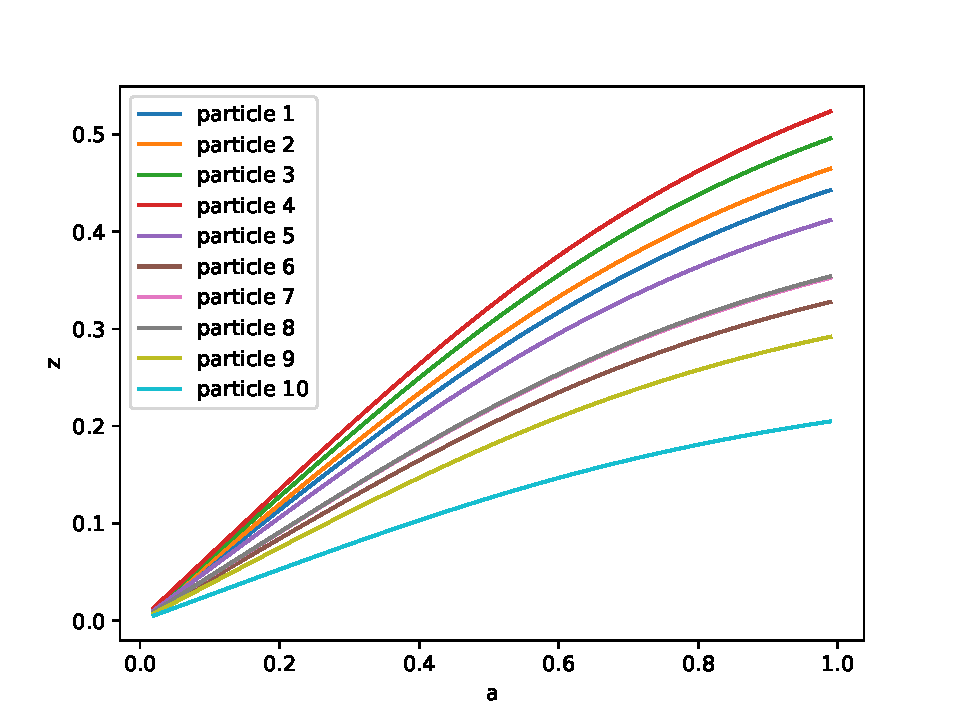
\includegraphics[width=14cm, height=9.5cm]{./Plots/4d_pos.pdf}
\caption{The z-positions of the first 10 particles against the scale factor.}
\end{figure}

\begin{figure}[!ht]
\centering
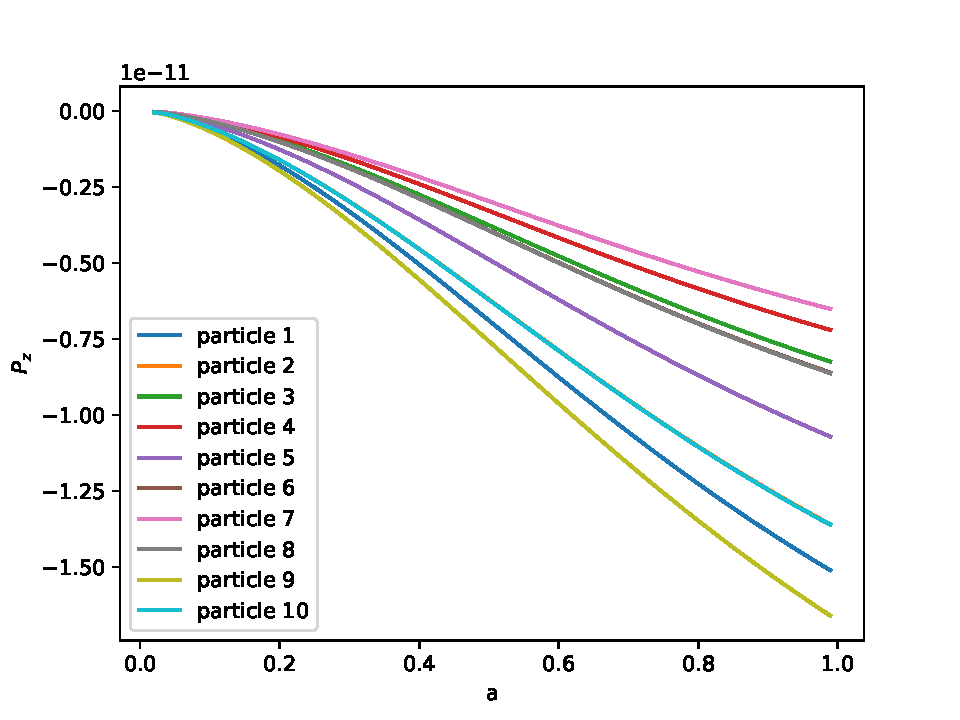
\includegraphics[width=14cm, height=9.5cm]{./Plots/4d_momentum.pdf}
\caption{The z-component of the momentum of the first 10 particles against the scale factor. }
\end{figure}
\end{quote}



\end{quote}




